% Shared text of the paper, used by main.tex (ACL, two columns, for submission)
% and preview.tex (one column, for reading). Edit the paper HERE.
% Values from the training and robustness analyses: results/analysis/ (scripts/analyze_all.py).
\title{One Alphabet Reform, Six Spellings:\\
How Uzbekistan's 2026 Latin Alphabet Affects LLM Tokenization, Accuracy and Training}

\author{Bilolbek Yoldoshxojayev \\
  Presidential School in Namangan, Uzbekistan \\
  \texttt{bilolbek424@gmail.com}}

\maketitle

\begin{abstract}
In 2026 Uzbekistan adopted a revised Latin alphabet that replaces the digraphs o\textquoteleft, g\textquoteleft, sh and ch with the single letters \"o, \u{g}, \c{s} and \c{c}. Uzbek is already typed with at least four different characters for the o\textquoteleft/g\textquoteleft{} mark, and is still widely written in Cyrillic. We build a parallel version of FLORES-200 and Belebele in these spellings using a lexicon-aware converter, and measure tokenizer fertility, reading-comprehension accuracy on six open LLMs, API cost, and the effect of training on each spelling. Relative to how Uzbek is commonly typed, the new alphabet changes token counts by $-3.0\%$ to $+1.3\%$. Yet it lowers accuracy in every model, by 3.1--9.6 percentage points, while apostrophe variants have no significant effect. This looks like a transition cost: fine-tuning Gemma 3 4B on 4 million characters of new-alphabet text closes its gap ($-6.8$ to $+0.3$ points). A small model trained from scratch shows no consistent difference between old and new spelling in tokens, training time, energy or predictive quality.
\end{abstract}

\section{Introduction}
On 10 September 2026 the Senate of Uzbekistan approved a law amending the Latin-based Uzbek alphabet, and the President signed it on 21 October 2026 \citep{legalalliance2026, gazeta2026}. The reform replaces four letter combinations with single letters (o\textquoteleft$\to$\"o, g\textquoteleft$\to$\u{g}, sh$\to$\c{s}, ch$\to$\c{c}), leaving 28 letters and one apostrophe; school textbooks are to be renewed in 2027--2031 \citep{legalalliance2026}. One stated motivation is digital: the o\textquoteleft{} mark is typed with several look-alike characters (U+02BB, ASCII ', the backtick, U+2019), so identical words are treated as different by software \citep{legalalliance2026}.

Whether the reform helps language technology is publicly disputed. The director of the Institute of Uzbek Language, Literature and Folklore, Maqsud Asadov, has said that two-character letters cause technical obstacles for digital systems and AI, while the philologist Komil Jalilov argues that it makes no difference to AI whether a letter takes one symbol or two \citep{sobirov2026}. Two recent reports measure token counts under the reform \citep{rozimatov2026, ibadullaev2026}, but we found no work that measures \emph{model accuracy} or training on the new alphabet, or compares it against the apostrophe variants that already exist in real text.

We ask: \textbf{RQ1} How do the spellings change tokenizer fertility? \textbf{RQ2} How do they change LLM accuracy? \textbf{RQ3} What does this mean for API cost and usable context? \textbf{RQ4} Does normalizing to one form remove the gaps? \textbf{RQ5} Does training on the new alphabet differ in cost or outcome from training on the old one?

Our contributions: (1) a parallel Uzbek version of FLORES-200 and Belebele, built with a lexicon-aware converter; (2) accuracy measurements of LLMs on the 2026 alphabet and on apostrophe variants; (3) a letter-level ablation separating \"o/\u{g} from \c{s}/\c{c}; (4) a paired old-versus-new training comparison, for fine-tuning and from scratch.

\section{Related Work}
\textbf{Tokenization and language variation.} Tokenizers allocate unequal numbers of tokens across languages \citep{petrov2023}, the tokenizer can matter as much as pretraining data for downstream performance \citep{rust2021}, and less common spellings can be split into more tokens, with tokenizer choices affecting downstream tasks \citep{wegmann2025}. \citet{ibadullaev2026} train SentencePiece and byte-level BPE tokenizers on Uzbek and find that the reform's token savings come from tokenizers splitting the apostrophe off the letter; with script splitting disabled the savings vanish. \citet{rozimatov2026} report modest, tokenizer-dependent savings for six widely used tokenizers, using direct letter replacement. Neither measures LLM accuracy or compares apostrophe variants.

\textbf{Uzbek evaluation.} TUMLU \citep{isbarov2025} evaluates LLMs on Turkic languages including Uzbek in Latin and Cyrillic and finds small, inconsistent script gaps. UzLiB \citep{shopulatov2025} is an Uzbek linguistic benchmark. \citet{sharipov2023uzbektagger} note that mixed apostrophe characters break Uzbek tokenization. \citet{kletz2026} study script awareness of language models on multi-script languages such as Serbian and Kazakh, not Uzbek.

\section{Data and Spelling Conditions}
\label{sec:data}
\textbf{Sources.} FLORES-200 \texttt{uzn\_Latn} devtest (1{,}012 sentences) and dev (997) \citep{nllb2022} for RQ1; Belebele \texttt{uzn\_Latn} \citep{bandarkar2024} (900 multiple-choice questions on 488 FLORES passages) for RQ2. Both are CC BY-SA 4.0 and written in 1995 Latin with the ASCII apostrophe (Belebele: 10{,}221 ASCII vs.\ 28 U+02BB). For RQ5, 106{,}658 FineWeb-2 \texttt{uzn\_Latn} documents \citep{fineweb2}, converted the same way, with no FLORES documents; 1 of 29{,}072 Belebele 8-grams occurs in this corpus.

\textbf{Conditions.} We first canonicalize every apostrophe-like character to U+02BB after o/g and to U+02BC (tutuq belgisi) elsewhere. From this we derive: \emph{okina} (official, canonical), \emph{ascii}, \emph{backtick} and \emph{rsquo} (both marks replaced by one character, as a single keyboard key produces them); \emph{new2026}; and \emph{cyrillic}. For the ablation we build \emph{only \"o\u{g}} and \emph{only \c{s}\c{c}}, which keep one half of the reform and undo the other. For RQ4 we add \emph{back-converted} (new2026 converted back to 1995 spelling) and \emph{mixed} (a seeded random apostrophe per word).

\textbf{Conversion to the 2026 alphabet.} Naive replacement wrongly converts foreign words (\emph{show}$\to$\emph{\c{s}ow}). We use YangiAlifbo\footnote{\url{https://github.com/BilolbekYoldoshxojayev/yangicha-alifbo}, commit \texttt{fdaafae}.}, an open-source converter with a 959{,}740-form lexicon, a 400+ suffix morphological analyzer, a 112{,}447-word foreign-word filter and character-level CNNs, run in strict mode through a batch CLI that also splits hyphenated and slash-joined words. Output is used as-is, without manual correction. On FLORES devtest it converts 5{,}183 of 5{,}288 candidate words; misses are mostly Uzbek-spelled foreign names (\emph{Polsha}, \emph{Vashington}). The author, a native speaker, hand-checked a sample after a first review by an AI assistant, finding 13 of 709 candidate words missed (1.8\%), errors in 7 of 100 FLORES sentences, and no false conversions.

\textbf{Cyrillic} is produced by a rule-based transliterator (digraphs, positional \emph{e}$\to$\cyrillic{э}/\cyrillic{е}, \emph{-tsiya}$\to$\cyrillic{-ция}); Latin-script names stay Latin. Some information is unrecoverable from 1995 Latin (soft sign, \cyrillic{ц} spelled \emph{s}), so this condition is transliterated, not native Cyrillic. The same hand-check found errors in 41 of 2{,}413 words (1.7\%), and in 19 of 100 FLORES sentences. All were in loanwords and names, such as \cyrillic{ц} written as \cyrillic{с} and missing soft signs.

\section{Experimental Setup}
\textbf{Tokenizers (RQ1).} o200k (GPT-4o/4.1/5), cl100k (GPT-4; identical to Phi-4), Llama 3.x, Qwen 2.5 (identical to Qwen 3), Gemma 3, Mistral Nemo (Tekken), DeepSeek V3, plus UTF-8 bytes. Fertility is tokens per word, with words counted once on the okina text. 95\% CIs: 1{,}000 sentence-level bootstrap resamples.

\textbf{Models (RQ2).} Gemma 3 4B (bf16 and 4-bit), Qwen 2.5 7B, Llama 3.1 8B, Qwen 3 8B, Gemma 3 12B and Mistral Nemo 12B, all instruction-tuned; models above 4B run with 4-bit NF4 quantization \citep{dettmers2023qlora} on one 12 GB GPU (RTX 4080 Laptop). A repeated run of 100 predictions was identical, with zero log-probability difference.

\textbf{Scoring.} Zero-shot, with an English prompt frame that is byte-identical across conditions. The prediction is the option letter (A--D) with the highest next-token log-probability; no sampling. On this raw frame the four letters receive 61--94\% of the probability mass depending on the model, so models do not always follow the format. We therefore repeat okina and new2026 with each model's chat template (95--100\%) and with an Uzbek frame written in the tested spelling.

\textbf{Statistics.} Paired comparisons against \emph{okina}: exact McNemar tests, Holm-corrected over the nine comparisons per model, and 95\% CIs from a cluster bootstrap over source articles (questions sharing a passage are not independent).

\textbf{Training (RQ5).} Both experiments use the same documents and seeds for each spelling, three seeds (42--44), with the order of spellings alternated. \emph{Fine-tuning:} LoRA ($r=16$) on 4-bit Gemma 3 4B, 1{,}133 documents (4M characters), then re-tested on Belebele. \emph{From scratch:} a 98M-parameter GPT-2-style model on 53{,}241 documents (200M characters), with a 16{,}000-entry byte-level BPE tokenizer that is either separate per spelling or shared (trained on both). Quality is validation bits per \emph{word}, because word counts are equal across spellings while token and character counts are not. Evaluation time is excluded from training time. In all training runs the GPU never reported thermal slowdown (maximum 66\,\textdegree{}C).

\section{Results}
\textbf{RQ1: tokens.} Figure~\ref{fig:tok} shows the change in tokens relative to \emph{okina}. Relative to ASCII, the form most Uzbek text actually uses, the new alphabet changes token counts by between $-3.0\%$ (Llama 3) and $+1.3\%$ (DeepSeek V3), and by $+1.1\%$ on o200k. The official U+02BB is the \emph{most} expensive Latin form for cl100k and Llama 3 (+5\% over ASCII), but the cheapest for Mistral Nemo. Cyrillic costs $+10\%$ to $+56\%$. The ablation splits the reform's effect: \"o/\u{g} alone save 2.0--7.7\% on six of seven tokenizers, while \c{s}/\c{c} alone change tokens by $-0.1\%$ to $+4.2\%$, plausibly because \emph{sh} and \emph{ch} are frequent letter pairs that subword vocabularies already merge. Results replicate on FLORES dev within 0.3 points.

\begin{figure}[t]
  \centering
  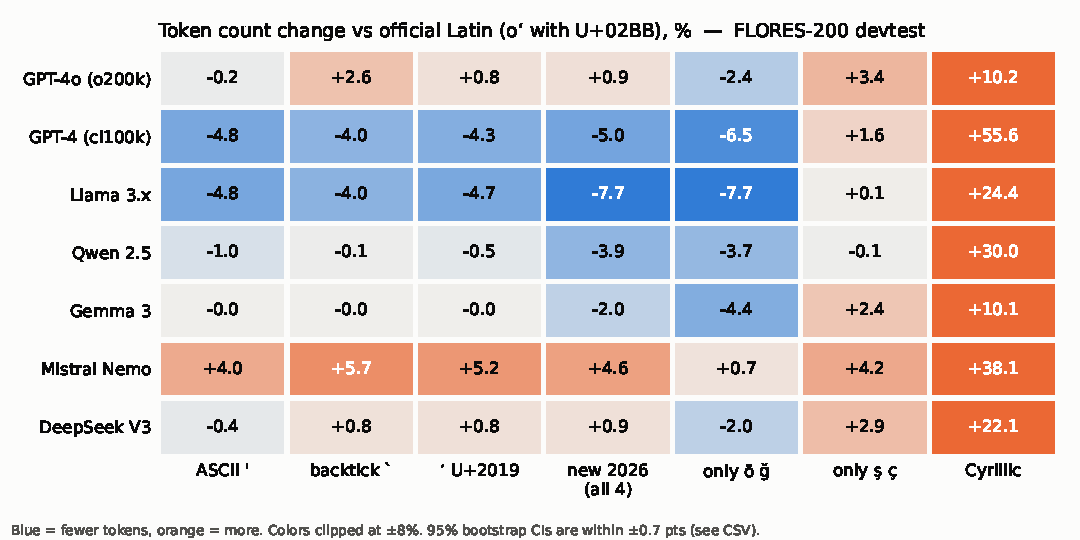
\includegraphics[width=\columnwidth]{flores_devtest_heatmap.pdf}
  \caption{Token change (\%) vs.\ official Latin on FLORES-200 devtest. Blue: fewer tokens; orange: more. All 95\% CIs within $\pm$0.7 points.}
  \label{fig:tok}
\end{figure}

\textbf{RQ2: accuracy.} Table~\ref{tab:acc} gives the main result. The 2026 alphabet lowers accuracy in every model, by 3.1 to 9.6 points, significant after correction in all seven runs. Within the Gemma 3 family the effect shrinks with size ($-7.4$ at 4B, $-3.1$ at 12B), but size alone does not protect a model: Mistral Nemo, also 12B, has the largest drop ($-9.6$). None of the 28 apostrophe comparisons (three variants and mixed) is significant after correction. Cyrillic is significantly worse in four of seven runs, up to $-18.6$ (Mistral Nemo). In the ablation, neither half of the reform alone reproduces the full drop, and in 5 of 7 runs \c{s}/\c{c} cost more accuracy than \"o/\u{g}, although \c{s}/\c{c} are the letters that do not save tokens.

\begin{table}[t]
\centering\small
\setlength{\tabcolsep}{3pt}
\begin{tabular}{lrrrrrr}
\toprule
Model & okina & ascii & new & \"o\u{g} & \c{s}\c{c} & cyr \\
\midrule
Gemma 3 4B & 64.0 & $-0.3$ & $\mathbf{-7.4}$ & $\mathbf{-3.1}$ & $\mathbf{-5.9}$ & $\mathbf{-4.7}$ \\
\quad 4-bit & 59.9 & $+0.4$ & $\mathbf{-6.8}$ & $-1.3$ & $\mathbf{-3.9}$ & $-2.6$ \\
Qwen 2.5 7B & 60.2 & $-0.6$ & $\mathbf{-4.7}$ & $-1.2$ & $-0.4$ & $\mathbf{-4.7}$ \\
Llama 3.1 8B & 69.1 & $+0.6$ & $\mathbf{-6.9}$ & $-2.4$ & $-3.0$ & $\mathbf{-8.7}$ \\
Qwen 3 8B & 69.7 & $+0.9$ & $\mathbf{-4.3}$ & $-1.8$ & $-1.1$ & $-3.3$ \\
Gemma 3 12B & 84.9 & $+1.0$ & $\mathbf{-3.1}$ & $-1.0$ & $-1.4$ & $-0.7$ \\
Mistral Nemo 12B & 74.7 & $+0.7$ & $\mathbf{-9.6}$ & $\mathbf{-3.8}$ & $\mathbf{-6.9}$ & $\mathbf{-18.6}$ \\
\bottomrule
\end{tabular}
\caption{Belebele accuracy (\%) with official Latin, and change in points for other spellings. Bold: significant after Holm correction (exact McNemar, $\alpha=0.05$). Backtick, \textquoteright{} and mixed omitted for space (all $|\Delta| \le 1.2$, none significant).}
\label{tab:acc}
\end{table}

\textbf{Robustness.} With the six 4-bit models the new-alphabet gap is negative under all three frames. It is significant for five of six models with the chat template ($-2.7$ to $-9.2$; Qwen 2.5 is not significant) and five of six with the Uzbek frame ($-1.8$ to $-9.8$; Gemma 3 4B is not). The Uzbek-frame result for Qwen 3 is weak, since only 27\% of its probability mass falls on the letters.

\textbf{Dose--response (exploratory).} Pooled over the six 4-bit models, the gap grows with the density of new letters: $-3.9$, $-6.1$ and $-7.7$ points across thirds of questions, a slope of $-0.98$ points per additional new letter per 100 letters (95\% CI $[-1.76, -0.26]$; $-0.92$ controlling for length). Five of six models have a negative slope, but only one has a CI excluding zero.

\textbf{RQ3: cost.} Because API price is linear in tokens, the token changes above are cost changes. With prices checked on 30 Oct 2026, one million Uzbek words cost \$3.28 (ASCII) vs.\ \$3.31 (new alphabet) of GPT-5 input; Cyrillic costs \$3.62. A 128k-token context holds about 48{,}900 Uzbek words with o200k in ASCII Latin and 48{,}300 in the new alphabet, but only 24{,}200 with cl100k in Cyrillic.

\textbf{RQ4: normalization.} Apostrophe variants, including random mixing, leave no significant gap to close. Back-converting new2026 removes the accuracy gap on our data: the change is at most 0.1 points in all seven runs, and answers match okina on at least 99.9\% of questions in the six 4-bit models. The round trip is not perfect (99.69\% of Belebele fields are identical; differences include all-caps forms such as \emph{AQSH}$\to$\emph{AQSh}). This tests our own conversion, not text written natively in the new alphabet.

\textbf{RQ5: training.} Table~\ref{tab:train} shows training cost and quality. Token counts differ little: $-1.5\%$ for Gemma's tokenizer with LoRA, and $+0.27\%$ (separate) and $+0.08\%$ (shared) from scratch. The new alphabet therefore brings no meaningful saving in our trained tokenizers either. Peak memory is identical (6.58 and 9.52 GB). Timing differences reflect machine state more than spelling. One from-scratch old-spelling run was 27\% slower, with lower GPU power and no thermal flag (cause unknown); without it, old and new take 27.9 and 28.0 minutes. LoRA throughput varied within spelling (378--426 tokens/s), and the one pair with equal throughput differs by 1.5\%, matching the token count. From scratch, the bits-per-word differences change sign across seeds and tokenizer modes and are within seed-to-seed spread, so we detect no quality difference with three seeds.

\begin{table}[t]
\centering\small
\setlength{\tabcolsep}{3pt}
\resizebox{\columnwidth}{!}{%
\begin{tabular}{llrrrr}
\toprule
Setup & Sp. & Tokens (M) & Min & Wh & Bits/word \\
\midrule
LoRA & old & 1.43 & $60.6 \pm 4.1$ & $75.8$ & $9.47 \pm 0.01$ \\
 & new & 1.41 & $56.4 \pm 1.3$ & $73.4$ & $10.01 \pm 0.00$ \\
Scratch, sep. & old & 43.73 & $31.3 \pm 6.0$ & $54.3$ & $12.11 \pm 0.17$ \\
 & new & 43.85 & $28.0 \pm 0.0$ & $52.3$ & $12.01 \pm 0.04$ \\
Scratch, shared & old & 44.74 & $28.6 \pm 0.0$ & $53.4$ & $11.96 \pm 0.17$ \\
 & new & 44.77 & $28.6 \pm 0.0$ & $53.4$ & $12.09 \pm 0.15$ \\
\bottomrule
\end{tabular}}
\caption{Training on old vs.\ new spelling: mean $\pm$ SD over three seeds. Bits per word on validation text in the same spelling.}
\label{tab:train}
\end{table}

Fine-tuning changes the accuracy gap. Mean over three seeds, on Gemma 3 4B (4-bit), the new-minus-old-text gap is $-6.8$ points $[-9.7, -4.0]$ for the base model, $-4.0$ $[-6.1, -1.9]$ after training on old spelling, and $+0.3$ $[-1.1, +1.8]$ after training on new spelling. On new-alphabet questions, the new-trained model beats the base by 5.1 points $[+2.6, +7.9]$ and the old-trained model by 3.5 $[+1.5, +5.6]$, significant in each seed after Holm correction. Accuracy of each model on its own spelling does not differ detectably ($-0.5$ $[-2.1, +1.2]$), and training on new spelling does not significantly hurt old-spelling accuracy compared with the base ($-2.0$ $[-4.3, +0.4]$). LoRA did not raise accuracy on old text above the base model, so this result concerns the gap between spellings, not overall skill.

\section{Discussion}
The reform's token savings are small and tokenizer-dependent, consistent with \citet{ibadullaev2026}. Its accuracy cost, by contrast, is consistent across models and prompt frames. Our training results point to distribution shift: current models saw little Uzbek written with \"o, \u{g}, \c{s}, \c{c}, and a small amount of such text closes the gap in the one model we tested. The cost therefore looks like a \emph{transition} cost that should shrink as new-alphabet text enters training data. From scratch, neither spelling has a clear advantage, which does not support strong claims in either direction in the public debate: on our evidence, the new letters neither make models cheaper to train nor harder to teach. For practitioners during the 2027--2031 transition, back-converting new-alphabet input to the 1995 spelling is a cheap fix for current models, and standardizing apostrophes is, on present evidence, not needed for accuracy.

\section*{Limitations}
New-alphabet and Cyrillic text are converted, not written by people; converter errors and unrecoverable Cyrillic distinctions may affect results, and our error rates come from one annotator, the author of the converter, working after a first AI review, so they are not independent and some errors may have been missed. Fine-tuning used the same converter as the test text, so the model may partly be learning that converter's output, and it was tested on one model only. Three seeds detect only large training effects. FLORES/Belebele are translated encyclopedic and news text. We test one task, zero-shot. We had limited GPU power, one 12 GB laptop GPU, so we test only open models up to 12B, mostly 4-bit quantized, fine-tune on 4M characters and train only a 98M-parameter model from scratch. Proprietary models (Claude, Gemini, GPT) are not evaluated. Mirrors of gated repositories were used for some models; exact revisions are logged. An early Llama run was discarded after a hash check found a corrupted weight file; reported numbers come from the repaired model. Accuracy runs started before the laptop's cooling settings were fixed, but only training timings depend on that, and those came after.

\section*{Ethics and Use of AI Assistants}
All benchmark data is public under CC BY-SA 4.0. The author conceived the study, defined its research questions, spelling conditions and rigor requirements, proposed the old-versus-new training comparison, built the YangiAlifbo converter, chose the benchmark, hand-checked the converted text samples, and reviewed the final paper. An AI assistant (Claude) wrote the evaluation and analysis code, ran the experiments, did a first review of the converted text samples, contributed to the detailed study design, and drafted the text. The author takes responsibility for the content.
\bibliography{references}
